\section{Les modules}
%\leconwithtoc

\subsection{Introduction}

\begin{frame}
	\begin{itemize}
	\item
	Outre le choix de noms de variables explicites et une indentation
	correcte, tout bon programmeur se doit de veiller à la clarté et la
	lisibilité de ses algorithmes.
	\item
	Il est courant que les lignes de codes de programmes se
	comptent en centaines ou en milliers.
	\item
	Lors de l’écriture d’un algorithme, on 
	conseille, dans un souci de lisibilité, qu’aucun des modules
	ne dépasse la longueur d’une vingtaine de lignes.
	\end{itemize}
\end{frame}

\begin{frame}{Illustration}
	Commençons par écrire l'algorithme qui donne le maximum de 2 nombres.

	\bigskip
	
	\cadre{
	\begin{pseudo}
	\LComment Lit deux nombres et affiche le maximum des deux.
	\Module{max2}{}{}
		\Decl a,b,max~: réels
		\Read a,b
		\If{a > b}
			\Let max \Gets a
		\Else
			\Let max \Gets b
		\EndIf
		\Write max
	\EndModule
	\end{pseudo}
	}
\end{frame}

\begin{frame}{Illustration}
	À partir de là, trouvons le maximum de 3 nombres.
	
	\bigskip
	
	Il existe plusieurs approches. 
	
	\bigskip
	
	Voyons celle-ci~:

	\bigskip
	
	\cadre{
	\begin{enumerate}
		\item Calculer le maximum des deux premiers nombres, soit temp
		\item Calculer le maximum de temp et du troisième nombre, ce qui donne le résultat.
	\end{enumerate}
	}

\end{frame}

\begin{frame}{Illustration}
	Sur base de cette idée, comment faire à présent
	pour introduire le calcul du maximum de 2 nombres dans l’algorithme
	calculant le maximum de 3 nombres ? 
\end{frame}

\begin{frame}{Illustration}

	Une solution consiste à
	«~copier-coller~» les lignes de code du module
	\textit{{max2}}	dans le module
	\textit{{max3}}, toutefois en adaptant son contenu 
	au contexte de ce module~: 
	
	\bigskip
	\begin{itemize}
	\item
	les nombres
	\textit{{a}}	et
	\textit{{b}}
	ne doivent plus être systématiquement lus 
	\item
	et la valeur du maximum ne
	doit plus être systématiquement affichée. 
	\end{itemize}
	
	\bigskip
	
	Ainsi \textit{{temp}}
	est calculé et ré-utilisé dans un calcul ultérieur.
\end{frame}

\begin{frame}{Illustration}

	Ceci donnerait~:

	\cadre{
	\begin{pseudo}
	\Module{max3}{}{}
		\LComment Lit trois nombres et affiche le maximum des trois.
		\Decl a, b, c, temp, max~: réels
		\Read a,b,c
		\If{a > b}
			\Let temp \Gets a
		\Else
			\Let temp \Gets b
		\EndIf
		\If{temp > c}
			\Let max \Gets temp
		\Else
			\Let max \Gets c
		\EndIf
		\Write max
	\EndModule
	\end{pseudo}
	}
\end{frame}

\begin{frame}{Illustration}
	Imaginons, par exemple, que l'on doive calculer le
	maximum de 4 ou même 5 nombres. 
	
	\bigskip
	
	Le résultat serait un code long et
	à l'allure répétitive. Une erreur serait vite arrivée et
	serait difficile à détecter.
	
	\bigskip
	
	L’idéal serait de 
	\begin{itemize}
	\item
	pouvoir garder deux modules séparés, conservant chacun
	leur spécificité (l’un calculant le maximum de deux nombres et l’autre
	le maximum de trois nombres) 
	\item
	mais de leur permettre de communiquer
	entre eux pour s’échanger des données ou des résultats de calculs. 
	\end{itemize}
	
	\bigskip
	
	Nous allons voir deux solutions.
\end{frame}

\subsection{Passage de paramètres}

\begin{frame}{passage de paramètres}
	Pour pouvoir faire communiquer les modules entre eux, 
	
	il faut les	équiper d’une «~\code{interface}~» 
	de transmission des variables appelée
	l’\code{en}-\code{tete} du module et qui contient une déclaration de
	variables qu’on appellera ici \code{parametres} du module. 
\end{frame}

\begin{frame}{passage de paramètres}
	\begin{itemize}
	\item
	Les variables accompagnées d’une flèche vers le bas ($\downarrow$) sont
	des \textbf{paramètres d’entrée} qui reçoivent des données au
	\textbf{début} de l’exécution du module (données qui ne doivent donc
	plus être lues) 
	\item
	tandis que celles accompagnées d’une flèche vers le
	haut ($\uparrow$) sont des \textbf{paramètres de sortie} qui permettent
	de renvoyer des résultats à l’\textbf{issue} de l’exécution du module
	(résultats qui ne doivent donc plus être affichés). 
	\end{itemize}
\end{frame}

\begin{frame}{Illustration}

	Par exemple, ceci donnerait pour le module \textit{max2}~:

	\bigskip
	
	\cadre{
	\begin{pseudo}
	\LComment Affiche deux nombres et sort le maximum des deux.
	\Module{max2}{a\In, b\In~: réels, max\Out~: réel}{}
		\If{a > b}
			\Let max \Gets a
		\Else
			\Let max \Gets b
		\EndIf
	\EndModule
	\end{pseudo}
	}
\end{frame}

\begin{frame}{Illustration}

	Pour faire appel aux services de ce module, il
	suffit à présent d’écrire son nom suivi d’un nombre de variables (ou,
	en entrée, d'expressions) en accord avec son entête. 
\end{frame}

\begin{frame}{Illustration}

	Montrons par un exemple comment le module
	\textit{{max3}}
	peut faire appel au module
	\textit{{max2}}~:

	\bigskip
	
	\cadre{
	\begin{pseudo}
	\LComment Lit trois nombres et affiche le maximum des trois.
	\Module{max3}{}{}
		\Decl a, b, c, temp, max~: réels
		\Read a, b, c
		\Stmt max2( a, b, temp )
		\Stmt max2( temp, c, max )
		\Write max
	\EndModule
	\end{pseudo}
	}
\end{frame}

\begin{frame}{Illustration}
	
	L’instruction
	\textit{{max2(a, b,
	temp)}} se déroule comme suit~:
	
	\begin{itemize}
	\item {
	{le contenu des variables
	}\textit{{a}}{
	et
	}\textit{{b}}{
	est affecté aux paramètres d’entrée
	}\textit{{a}}{
	et
	}\textit{{b}}{
	du module
	}\textit{{max2}}{,
	puis ce module peut entrer en action~;}}
	\item {
	{à l’issue du module
	}\textit{{max2}}{,
	la valeur du paramètre de sortie
	}\textit{{max}}{
	est communiquée à la variable
	}\textit{{temp}}{,
	qui contient à présent le maximum de
	}\textit{{a}}{
	et
	}\textit{{b}}{.}}
	\end{itemize}
\end{frame}

\begin{frame}{Illustration}
	
	L’instruction \textit{max2(temp, c, max)}
	se déroule comme suit~:
	
	\begin{itemize}
	\item {
	{le contenu des variables
	}\textit{{temp}}{
	et
	}\textit{{c}}{
	est affecté aux paramètres d’entrée
	}\textit{{a}}{
	et
	}\textit{{b}}{
	du module
	}\textit{{max2}}{,
	puis ce module peut entrer en action~;}}
	\item {
	{à l’issue du module
	}\textit{{max2}}{,
	la valeur du paramètre de sortie
	}\textit{{max}}{
	est communiquée à la variable
	}\textit{{max}}{,
	qui contient à présent le maximum des 3 nombres de départ.}}
	\end{itemize}

	{Il est évident que la présence de ces deux
	instructions dans le module
	}\textit{{max3}}{
	implique la présence du module
	}\textit{{max2}}{
	«~aux alentours~» du premier, c’est-à-dire que ces deux modules doivent
	se trouver sur le même support d’écriture de
	l'algorithme complet.}
\end{frame}

\begin{frame}{Remarques}
	\begin{itemize}
	\item {
	{un paramètre peut être à la fois paramètre
	d’entrée et de sortie~; on le fait suivre alors de la double flèche
	}{$\uparrow \downarrow$}{~;}}
	\item {
	si tous les paramètres sont en entrée, on peut omettre les flèches;}
	\item {
	la présence de ces paramètres n’est pas obligatoire, on peut envisager
	un module sans paramètre de sortie (par ex. un module qui reçoit en
	entrée un nombre et dont la seule fonction est de l’afficher à
	l’écran), ou inversement sans paramètre d’entrée (un module qui simule
	un lancer de dé, et renvoie en paramètre une valeur aléatoire entre 1
	et 6)~;}
	\end{itemize}
\end{frame}

\begin{frame}{Remarques}
	\begin{itemize}
	\item {
	{pour appeler correctement un module, il faut
	fournir des noms de variables, des expressions ou des constantes
	}{\textbf{en même
	nombre}}{ et en même ordre que les paramètres
	du module~;}}
	\item {
	en outre, les types des variables doivent correspondre entre l’appel et
	l’en-tête du module~;}
	\item {
	ne peut être affectée à un paramètre d’entrée du module qu’une
	constante, une expression ou une variable préalablement affectée~;}
	\end{itemize}
\end{frame}

\begin{frame}{Remarques}
	\begin{itemize}
	\item {
	à un paramètre de sortie d’un module doit toujours correspondre une
	autre variable, jamais une constante ou une expression~;}
	\item {
	il faut s’assurer qu’à l’issue du module, tous les paramètres de sortie
	aient été affectés lors de l’exécution de ce module.}
	\end{itemize}

\end{frame}

\subsection{Variables locales}

\begin{frame}{variables locales}
	\begin{itemize}
	\item
	Dans le cadre de ce cours d’algorithmique,
	nous n’envisagerons que l’utilisation de 
	\textbf{variables locales}. 
	\item
	Toute variable est \textbf{locale} au module 
	dans lequel elle apparait, ce qui veut dire que son existence
	est ignorée en dehors de ce module. 
	\item
	Nous n’envisageons donc pas ici l’utilisation déconseillée de 
	\textbf{variables globales} 
	(variables dont le contenu est reconnu 
	par tous les modules d’un programme).
	\item
	Précisons qu'une variable locale est aussi
	\textbf{dynamique}, c’est-à-dire qu’un emplacement en mémoire lui est
	réservé durant l’exécution du module où elle est déclarée. Une fois
	l’exécution terminée, cet emplacement est récupéré en mémoire.
	\end{itemize}
\end{frame}

\begin{frame}{variables locales}
	\begin{itemize}
	\item
	Plutôt qu’une restriction, cette propriété est
	une aide confortable au programmeur~: si, de
	façon fortuite, des variables appartenant à des modules différents
	possédaient le même nom, il n’y aurait pas d’interférence entre ces
	variables, ni confusion possible de leur
	contenu.
	\item
	Notons au passage que les variables déclarées dans l’entête du module ne
	doivent plus l’être dans la partie «~déclaration de variables~» de ce
	module. Mais toutes les variables utilisées dans un module doivent être
	déclarées, soit dans son entête, soit dans sa déclaration. Le
	non-respect de cette règle provoquerait une erreur d’exécution.
	\end{itemize}
\end{frame}

\begin{frame}{exemple}
	\cadre{
	\begin{pseudo}
	\LComment Lit trois nombres positifs et affiche le maximum des trois.
	\Module{max3}{}{}
		\Decl a, b, c, temp, max~: réels
		\Stmt lirePositif(a)
		\Stmt lirePositif(b)
		\Stmt lirePositif(c)
		\Stmt max2(a, b, temp)
		\Stmt max2(temp, c, max)
		\Write max
	\EndModule
	\end{pseudo}
	}
\end{frame}

\begin{frame}{exemple}
	\cadre{
	\begin{pseudo}
	\LComment Lit un nombre, le sort s'il est positif et sinon lance une erreur.
	\Module{lirePositif}{a\Out~: réel}{}
		\Read a
		\If{a < 0}
			\Error Le nombre n'est pas positif !
		\EndIf
	\EndModule
	\end{pseudo}
	}
\end{frame}

\begin{frame}{exemple}
	\cadre{
	\begin{pseudo}
	\LComment Affiche deux nombres et sort le maximum des deux.
	\Module{max2}{a\In, b\In~: réels, max\Out~: réel}{}
		\If{a > b}
			\Let max \Gets a
		\Else
			\Let max \Gets b
		\EndIf
	\EndModule
	\end{pseudo}
	}
\end{frame}

\subsection{Module renvoyant une valeur}

\begin{frame}{valeur en retour}
	Un deuxième type de module est le 
	\textbf{module renvoyant une valeur}. 
	
	(On désigne aussi ce type de modules par le terme \textbf{fonction}).
	
	\bigskip
	
	Son entête est du type suivant~:

	\bigskip
	
	\cadre{
	\begin{pseudo}
	\ModuleSign{exemple }{var1\In~: type1, var2\In~: type2, \dots, varN\In~: typeN}{typeRes}
	\end{pseudo}
	}
\end{frame}

\begin{frame}{valeur en retour}
	Il se distingue du module précédemment étudié par la flèche de renvoi à
	droite, et possède les particularités suivantes~:

	\begin{itemize}
	\item {
		{ce module renvoie
		}{\textbf{une}}{
		}{\textbf{valeur}}{
		}{\textbf{qui n’est pas affectée à une variable
		de
		}}{\textbf{sortie~}}{;}}
	\item {
		{à droite de la flèche de renvoi ne se trouve
		donc pas le nom d’un paramètre de sortie, mais le
		}{\textbf{type}}{ de la
		valeur renvoyée~;}}
	\item {
		\textit{{typeRes}}{
		est le type de la valeur renvoyée~; 
		
		en théorie, ce peut être 
		\begin{itemize}
		\item
		un type
		simple (entier, réel, booléen, chaine, caractère), 
		\item
		un type structuré,
		\item
		un tableau 
		\item
		ou même un objet (ces types seront vus dans les chapitres 
		suivants). 
		\end{itemize}
		En pratique il conviendra de s’en tenir aux limitations 
		du langage utilisé~;}}
	\end{itemize}
\end{frame}

\begin{frame}{valeur en retour}
	\begin{itemize}
	\item {
		\textit{{var1}}{,
		...,
		}\textit{{varN}}{
		sont les paramètres du module (aussi appelés
		}{\textbf{arguments}}{)
		; ce sont, le plus souvent, des paramètres d’entrée, les paramètres de
		sortie }{étant plus rares dans ce type de
		module~;}}
	\item {
		ces arguments deviennent automatiquement des variables locales du module
		; déclarées dans son en-tête, elles ne doivent plus l’être dans la
		partie déclarative~;}
		\end{itemize}
\end{frame}

\begin{frame}{valeur en retour}
	\begin{itemize}
	\item {
		{la valeur renvoyée est définie à la fin du
		module via la primitive
		}\textit{{retourner}}{
		}\textit{{résultat}}{,
		où
		}\textit{{résultat}}{
		est une variable (ou plus généralement une expression) de type
		}\textit{{typeRes}}{
		;}}
	\item {
		pour appeler ce type de module, on utilise son nom \textit{comme celui
		d’une variable} ou dans une expression apparaissant 
		dans le module appelant, mais jamais à gauche du signe
		d’affectation.}
	\end{itemize}
	
	\bigskip
	
	Comme précédemment, il faut veiller, lors de l’appel de ce 
	type de module, à ce que le nombre d’arguments ainsi que leur type
	correspondent à ceux spécifiés dans l’entête.
\end{frame}

\begin{frame}{exemple}
	Pour exemple, transformons une fois de plus la
	dernière version de notre algorithme.
	
	\bigskip
	
	\cadre{
	\begin{pseudo}
	\LComment Lit trois nombres positifs et affiche le maximum des trois.
	\Module{max3}{}{}
		\Decl a, b, c, temp, max~: réels
		\Let a \Gets lirePositif()
		\Let b \Gets lirePositif()
		\Let c \Gets lirePositif()
		\Let temp \Gets max2(a, b)
		\Let max  \Gets max2(temp, c)
		\Write max
	\EndModule
	\end{pseudo}
	}
\end{frame}

\begin{frame}{exemple}
	\cadre{
	\begin{pseudo}
	\LComment Lit un nombre, le retourne s'il est positif et sinon lance une erreur.
	\Module{lirePositif}{}{réel}
		\Decl a~: réel
		\Read a
		\If{a < 0}
			\Error Le nombre n'est pas positif !
		\EndIf
		\Return a
	\EndModule
	\end{pseudo}
	}
\end{frame}

\begin{frame}{exemple}
	\cadre{
	\begin{pseudo}
	\LComment Affiche deux nombres et retourne le maximum des deux.
	\Module{max2}{a\In, b\In~: réels}{réel}
		\Decl max~: réel
		\If{a > b}
			\Let max \Gets a
		\Else
			\Let max \Gets b
		\EndIf
		\Return max
	\EndModule
	\end{pseudo}
	}
\end{frame}

\begin{frame}{exemple}
	L'écriture avec une valeur de retour permet une
	écriture plus compacte~:

	\bigskip
	
	\cadre{
	\begin{pseudo}
	\LComment Lit trois nombres positifs et affiche le maximum des trois.
	\Module{max3}{}{}
		\Decl a, b, c, max~: réels
		\Let a \Gets lirePositif()
		\Let b \Gets lirePositif()
		\Let c \Gets lirePositif()
		\Let max  \Gets max2(max2(a, b), c)
		\Write max
	\EndModule
	\end{pseudo}
	}
\end{frame}

	\bigskip
	
\begin{frame}{exemple}
	ou encore (mais on perd un peu en clarté)~:

	\bigskip
	
	\cadre{
	\begin{pseudo}
	\LComment Lit trois nombres positifs et affiche le maximum des trois.
	\Module{max3}{}{}
		\Decl a, b, c~: réels
		\Let a \Gets lirePositif()
		\Let b \Gets lirePositif()
		\Let c \Gets lirePositif()
		\Write max2(max2(a, b), c)
	\EndModule
	\end{pseudo}
	}

	\bigskip
	
	ou même (et là, ce n'est plus du tout lisible !)~:

	\bigskip
	
	\cadre{
	\begin{pseudo}
	\LComment Lit trois nombres positifs et affiche le maximum des trois.
	\Module{max3}{}{}
		\Write max2(max2(lirePositif(), lirePositif()), lirePositif())
	\EndModule
	\end{pseudo}
	}
\end{frame}

\subsection{Un exemple complet}

\begin{frame}{Écart entre 2 moments}
	Étant donné deux moments dans une journée donnés chacun par trois
	nombres (heure, minute, seconde), 
	
	écrire un algorithme qui calcule et
	affiche le délai écoulé entre ces deux moments en heure(s), minute(s),
	seconde(s) 
	
	sachant que le deuxième moment donné est chronologiquement
	postérieur au premier.
\end{frame}

\begin{frame}{Écart entre 2 moments}
	Le problème n'est pas simple. 
	
	\bigskip
	
	On pourrait se dire qu'il suffit de soustraire les heures, 
	les minutes et les secondes.

	\bigskip
	
	Ainsi, pour l'écart entre
	1h22'23'' et
	3h34'56'', on
	calcule 3h-1h=2h;
	34'-22'=12' et
	56''-23''=33''
	ce qui donne un écart de
	2h12'33''.

	\bigskip
	
	Mais il s'agit là d'un cas favorable
	sans résultat négatif. 
	
	\bigskip
	
	Si une des soustractions est négative, comme par
	exemple pour l'écart entre
	1h22'23'' et
	3h11'12'', de
	simples soustractions ne suffisent pas.
\end{frame}

\begin{frame}{Écart entre 2 moments}
	Rappelons-nous que nous
	avons déjà écrit des algorithmes proches de ce problème dans les
	exercices du chapitre sur les algorithmes séquentiels. 
	
	\bigskip
	
	Plus précisément~:

	\bigskip
	
	\cadre{
	\begin{pseudo}
		\ModuleSign{heuresEnSecondes}{}{}
		\ModuleSign{secondesEnHeures}{}{}
	\end{pseudo}
	}
\end{frame}

\begin{frame}{Écart entre 2 moments}
	L'idée est de tout convertir en
	secondes car alors la soustraction est simple. 
	
	\bigskip
	
	Le résultat est alors
	reconverti en heures-minutes-secondes.

	\begin{center}
	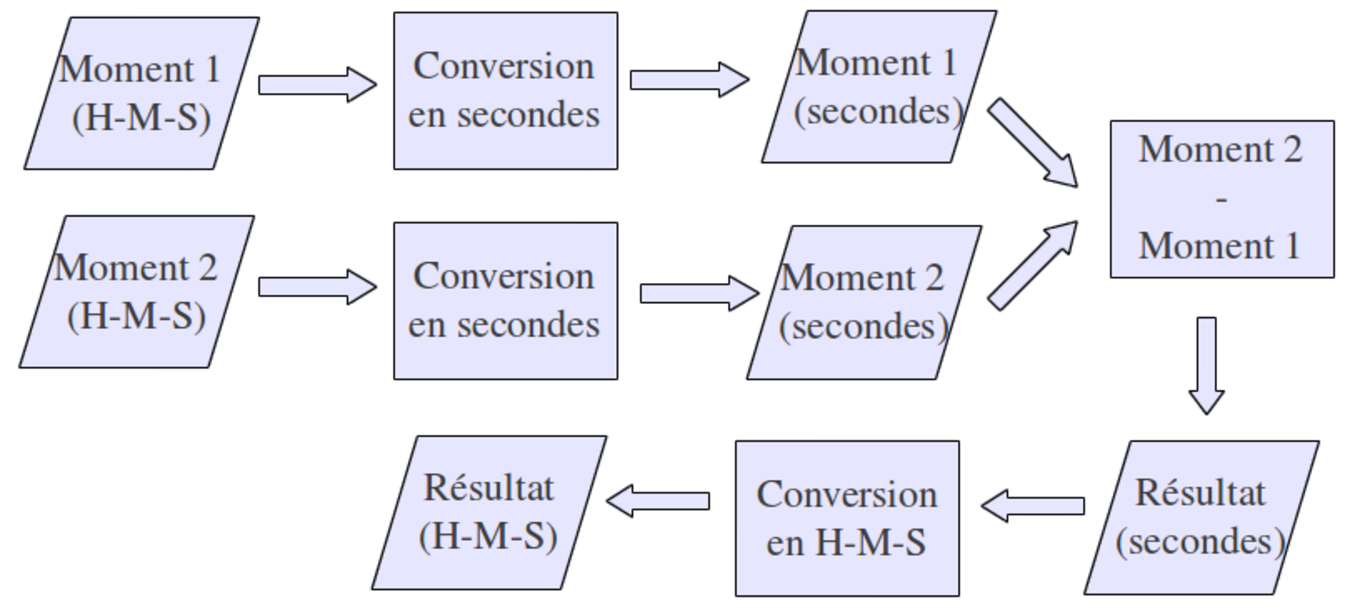
\includegraphics[width=0.8\textwidth]{image/module-conversion}
	\end{center}
\end{frame}

\subsubsection{Conversion en secondes}

\begin{frame}{Écart entre 2 moments}
	Une des sous-tâches est donc la conversion en secondes
	d'un moment exprimé en heures-minutes-secondes
	(h-m-s). 
	
	\bigskip
	
	Il nous faut adapter la solution trouvée pour
	l'exercice du chapitre sur les algorithmes séquentiels
	car il n'est pas question ici que les données soient
	lues ni que le résultat soit écrit~; 
	
	\bigskip
	
	l'interaction ne
	se fait pas avec l'utilisateur mais avec le module
	principal qui va l'utiliser.
\end{frame}

\begin{frame}{Écart entre 2 moments}
	La première question à se poser est donc celle des paramètres~:

	\bigskip
	
	\begin{itemize}
	\item 
		Quelles sont les données dont a besoin l'algorithme
		pour travailler ?
	\item 
		Quels résultats fournit-il ?
	\end{itemize}
\end{frame}

\begin{frame}{Écart entre 2 moments}
	Dans notre cas, la réponse est simple~:

	\bigskip
	
	\begin{itemize}
	\item {
		Les données sont le moment à convertir en secondes. 
		
		Ce moment est
		représenté par trois entiers~: les heures, les minutes et les secondes
		;}
	\item {
		Le résultat est le moment converti en secondes. 
		
		Il est représenté par un entier.}
	\end{itemize}
\end{frame}

\begin{frame}{Écart entre 2 moments}
	Lorsque le résultat est représenté par une seule donnée, on a le choix
	entre un paramètre en sortie~:

	\bigskip
	
	\cadre{
	\begin{pseudo}
		\LComment Affiche trois entiers~: des heures, des minutes et des secondes et sort le nombre de secondes correspondant.
		\ModuleSign{hmsVersSec}{h\In, m\In, s\In, secondes\Out~: entiers}{}
	\end{pseudo}
	}
	
	\bigskip
	
	ou une valeur de retour~:

	\bigskip
	
	\cadre{
	\begin{pseudo}
		\LComment Affiche trois entiers~: des heures, des minutes et des secondes et retourne le nombre de secondes correspondant.
		\ModuleSign{hmsVersSec}{h\In, m\In, s\In~: entiers}{entier}
	\end{pseudo}
	}
\end{frame}

\begin{frame}{Écart entre 2 moments}
		Dans de pareils cas, 
	on privilégie souvent la valeur de retour car cela
	facilite l'écriture lors de l'appel.

	\bigskip
	
	L'algorithme s'écrit alors~:

	\bigskip
	
	\cadre{
	\begin{pseudo}
	\LComment Affiche trois entiers~: des heures, des minutes et des secondes 
	\LComment et retourne le nombre de secondes correspondant.
		\Module{hmsVersSec}{h\In, m\In, s\In~: entiers}{entier}
			\Decl secondes~: entier \RComment {À déclarer puisque ce n'est pas un paramètre}
			\Let secondes \Gets  h * 3600 + m * 60 + s
			\Return secondes
		\EndModule
	\end{pseudo}
	}
\end{frame}

\begin{frame}{Écart entre 2 moments}
	ou de manière équivalente mais plus concise~:

	\bigskip
	
	\cadre{
	\begin{pseudo}
	\LComment Affiche trois entiers~: des heures, des minutes et des secondes 
	\LComment et retourne le nombre de secondes correspondant.
		\Module{hmsVersSec}{h\In, m\In, s\In~: entiers}{entier}
			\Return h * 3600 + m * 60 + s
		\EndModule
	\end{pseudo}
	}
\end{frame}

\subsubsection{Conversion en heures-minutes-secondes}

\begin{frame}{Conversion en heures-minutes-secondes}
	À la fin de notre algorithme, il nous faudra reconvertir un résultat
	exprimé en secondes sous la forme heures-minutes-secondes. 
	
	\bigskip
	
	À nouveau,
	on a déjà résolu ce problème dans le chapitre sur les algorithmes
	séquentiels. 
	
	\bigskip
	
	Mais il faut l'adapter à
	l'usage de paramètres.
\end{frame}

\begin{frame}{Conversion en heures-minutes-secondes}
	\begin{itemize}
	\item {
		Quelles sont les données ? 
		
		Une seule, le moment exprimé en secondes}
		
	\bigskip
	
	\item {
		Quels sont les résultats calculés par le module ? 
		
		Ce même moment exprimé
		en heures-minutes-secondes. 
		
		Trois entiers sont requis ce qui fait que
		le choix entre un paramètre en sortie et une valeur de retour ne se
		pose pas ici~; 
		
		impossible d'utiliser une valeur de
		retour (qui doit être unique)~; 
		
		on doit utiliser des paramètres en
		sortie.}
	\end{itemize}
\end{frame}

\begin{frame}{Conversion en heures-minutes-secondes}
	Ce qui donne~:

	\bigskip
	
	\cadre{
	\begin{pseudo}
		\LComment Affiche un nombre de secondes et sort les heures, les minutes et les secondes correspondant.
		\Module{secVersHMS}{secondes\In, s\Out, m\Out, s\Out~: entiers}{}
			\Let h \Gets secondes DIV 3600
			\Let m \Gets (secondes MOD 3600) DIV 60
			\Let s \Gets secondes MOD 60
		\EndModule
	\end{pseudo}
	}
\end{frame}

\subsubsection{Solution}

\begin{frame}{Solution}
	À présent, on a tout pour écrire la solution à notre problème

	\bigskip
	
	\cadre{
	\begin{pseudo}
		\LComment Lit deux moments (h-m-s) et affiche le moment de la différence entre les deux.
		\Module{différenceEntreHeures}{}{} \RComment Pas de paramètres !
			\Decl h1, m1, s1, h2, m2, s2~: entiers \RComment Les 2 moments à soustraire
			\Decl secondes1, secondes2~: entiers \RComment Ces 2 moments en secondes
			\Decl diffSecondes~: entier \RComment La différence en secondes
			\Decl diffH, diffM, diffS~: entiers \RComment La différence en H-M-S
			\Read h1, m1, s1, h2, m2, s2
			\Let secondes1 \Gets hmsVersSec( h1, m1, s1 )
			\Let secondes2 \Gets hmsVersSec( h2, m2, s2 )
			\Let diffSecondes \Gets secondes2 – secondes1
			\Stmt secVersHMS( diffSecondes, diffH, diffM, diffS )
			\Write diffH, diffM, diffS
		\EndModule
	\end{pseudo}
	}
\end{frame}

\begin{frame}{Solution}
	Dans la solution ci-dessus, 
	quelle est ou quelles sont la/les variable(s) locale(s) 
	dont on pourrait se passer moyennant une réécriture de
	l'algorithme ?
\end{frame}

\subsection{Blocs}

\begin{frame}{Blocs}
	\begin{itemize}
	\item
	Un bloc est l’écriture d’une portion de module
	à l’extérieur de celui-ci. C’est un simple
	{\textit{déplacement}}
	de lignes de codes vers un autre endroit du texte de
	l'algorithme.
	
	\bigskip
	
	\item
	La raison de découper un module en blocs
	peut être le souci de clarifier un algorithme en le découpant en étapes
	bien distinctes.
	
	\bigskip
	
	\item
	Les variables
	d’un bloc ne sont donc pas des variables locales du bloc dans lequel
	elles apparaissent, mais bien des variables locales du module auquel
	appartient ce bloc.
	\end{itemize}
\end{frame}

\begin{frame}{Blocs}
	\begin{itemize}
	\item
	L’appel de l’exécution des instructions se trouvant
	dans un bloc est similaire à celui d’un module avec paramètres, on
	écrit simplement le nom du bloc comme s’il s’agissait d’une
	instruction.
	\end{itemize}
\end{frame}

\begin{frame}{Blocs}
	Pour exemple, le module additionnerFractions (première version dans le
	chapitre 3) pourrait se découper ainsi~:

	\bigskip
	
	\cadre{
	\begin{pseudo}
	\LComment Lit les contenus de 2 fractions et affiche leur somme
		\Module{additionnerFractions}{}{}
			\Stmt déclaration
			\Stmt lectureDonnées
			\Stmt calculs
			\Stmt écritureRésultat
		\EndModule
	\end{pseudo}
	}
\end{frame}

\begin{frame}{Blocs}
	\cadre{
	\begin{pseudo}
	\Block{déclaration}
		\Decl num1, den1, num2, den2, numRes, denRes~: entiers
	\EndBlock
	\end{pseudo}
	}

	\bigskip
	
	\cadre{
	\begin{pseudo}
	\Block{lectureDonnées}
		\Read num1, den1, num2, den2
	\EndBlock
	\end{pseudo}
	}
\end{frame}

\begin{frame}{Blocs}
	\cadre{
	\begin{pseudo}
	\Block{calculs}
		\Let numRes \Gets num1 * den2 + num2 * den1
		\Let denRes \Gets den1 * den2
	\EndBlock
	\end{pseudo}
	}

	\bigskip
	
	\cadre{
	\begin{pseudo}
	\Block{écritureRésultat}
		\Write numRes, "/", denRes \RComment la fraction n'est pas simplifiée
	\EndBlock
	\end{pseudo}
	}
\end{frame}

\subsection{Qu'est-ce qu'un algorithme de qualité ?}

\begin{frame}{Algorithme de qualité}
	\begin{itemize}
	\item
	Nous voulons tous produire du code de qualité mais
	qu'est-ce que cette notion recouvre vraiment ?
	\item
	Qu'est-ce qui permet de juger de la qualité
	d'un code ? 
	\item
	De nombreux critères existent. 
	\end{itemize}
	
	\bigskip
	
	Citons ici,
	parmi les plus pertinents, ceux qui sont le plus liés à ce
	cours.
\end{frame}

\begin{frame}{Algorithme de qualité}
	\begin{itemize}
	\item
		La \textbf{validité}~: le code doit
	réaliser les tâches pour lesquelles 
	il a été écrit, même dans tous les
	cas particuliers imaginés.
	
	\bigskip
	
	\item 
		L'\textbf{extensibilité} (ou évolutivité)~:
	le code doit être écrit de telle sorte qu'un changement
	mineur dans le problème n'implique
	qu'un changement mineur dans le code.
	
	\bigskip
	
	\item
		La \textbf{réutilisabilité}~: c'est
	la capacité de réutiliser 
	un bout de code d’un projet dans un autre projet de 
	façon aisée et sûre.
	\end{itemize}
\end{frame}

\begin{frame}{Algorithme de qualité}
	\begin{itemize}
	\item
		La \textbf{lisibilité}~: 
		
	Au niveau global, on doit facilement comprendre la structure
	générale du code afin de pouvoir aisément comprendre où se trouve 
	la portion de	code qui nous intéresse. 
	
	Au niveau local, on doit pouvoir comprendre
	aisément chaque bout de code.
	
	\bigskip
	
	\item 
		L'\textbf{efficience}~: 
	ce critère s'intéresse à la bonne utilisation des
	ressources informatiques. Est-ce que le programme va tourner
	suffisamment vite, utiliser peu de mémoire ?
	\end{itemize}
\end{frame}
